The Kubernetes infrastructure can easily adjust its size according to the expected load.
Each workload is also adaptable to load peaks:
so far we're exploiting PHP-FPM's autoscaling capacity by scheduling server pods with fewer requirements than their memory limits
(under the assumption that load is bursty and uncorrelated between websites)
\footnote{So far we haven't found the Horizontal Pod Autoscaler useful, because the traffic on most "standard" QoS websites is too low to warrant multiple pods.}.
Nevertheless, we performed an experiment to measure the expected baseline resource consumption
\footnote{The server pod's memory needs to satisfy each website's Quality of Service requirements.
CPU in the CERN cloud is virtual and shared, so we don't take it into account when scheduling.}
and compare against the physical infrastructure, which, as we'll show, was overprovisioned.

We need a resource estimate to size the Kubernetes infrastructure so that it can handle the same baseline load as the physical infrastructure.
To understand the baseline load and the resources needed to handle it, we define Quality of Service (QoS) classes based on required throughput
that needs to be handled with a stable response latency.
We perform a stress test to emulate the throughput and define the appropriate baseline resources.

\subsection{Service level objectives}

\begin{figure}[t]
\centering
\captionsetup{justification=centering,margin=0.3cm}
\vspace{-2em}
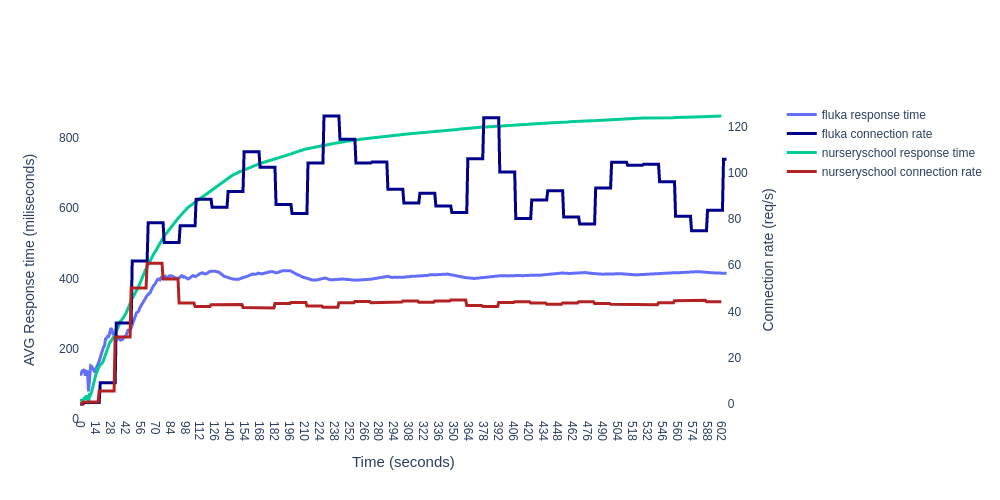
\includegraphics[width=1.1\linewidth]{figures/experiment-figures/critical_run.png}
\caption{\emph{Stress test for the Critical QoS}.
The right Y-axis shows the load for {\color[HTML]{b22222} \texttt{nurseryschool}} and {\color[HTML]{0000A0} \texttt{fluka}}.
The left Y-axis shows the response time (average over simultaneous requests) for {\color[HTML]{23CDCD} \texttt{nurseryschool}} and {\color[HTML]{636efa} \texttt{fluka}}.}
\label{stress_usage}
\vspace{-2em}
\end{figure}

To define the load each QoS class needs to handle, we use the physical infrastructure as starting point (fig. \ref{fig:website_bandwidth}).
Throughput peaked on the most popular website at around 16000 requests per hour, which averages on 4.4 requests per second.
We define 3 QoS classes, which serve as Service Level Objectives (SLO), against the Service Level Indicator (SLI) of response latency under load.
Because the latency depends on the complexity of each website, which is in the hands of the website admins and not the infrastructure,
the SLO is met \emph{not by defining a set value of the SLI, but by asserting that the SLI be stable}
\footnote{Stability is interpreted as the latency settling to a fixed value after some time with steady load}.
The 3 QoS classes are:

\begin{itemize}
    \item \textbf{Critical}: the most popular websites and therefore the most important to have high availability and request throughput (see section \ref{sec-load}).
    They need to handle 30 requests per second (around 8 times the average on peak usage).
    \item \textbf{Standard}: these websites usually don't handle as much traffic and therefore don't need to have high request throughput.
    They need to handle 5 requests per second. 
    \item \textbf{Test}: as in the name itself, these websites are used by website managers to test new features, and therefore are used by testers and developers.
    They only need to handle 1 request per second.
\end{itemize}
%- entire infra: 250 req/sec
%- critical website: 35 req/sec
%- standard website: 5-10 req/sec % TODO set final value
%- test website: 2 max threads

%- Find configuration that is able to handle specified req/sec load
%- Two Graphs (1 for critical and 1 normal), showing AVG response time plots + Request per second plots
%- See the Resources usage for each configuration
%- Make an estimation of total resources , note that critical websites will have $(MAX_LOAD) + 2(IDLE_LOAD)$ since they will have 3 pods

%Total number of Critical websites: 20
%Total number of Standard websites: 600
%Total number of Test websites: 500
%- Make an estimation of total infra resources ( sum to the estimation of total resources with openshift-* elements)

% #### Resources used in the physical infra:
% - Memory: 2TB
% - CPU: 512

\subsection{Stress test}

\begin{wraptable}{r}{.53\textwidth}
    \centering
    \begin{subtable}{0.5\textwidth}
        \begin{tabular}{|l|ll|ll}
        \cline{1-3}
        \textbf{website} & \multicolumn{1}{l|}{\textbf{Stress (req/s)}} & \textbf{Response (ms)} &  &  \\ \cline{1-3}
        nurseryschool    & 10                                           & 510                    &  &  \\ \cline{1-1}
        fluka            & 26                                           & 570                    &  &  \\ \cline{1-3}
        \end{tabular}
    \caption{Test}
    \end{subtable}
    \begin{subtable}{0.5\textwidth}
        \begin{tabular}{|l|ll|ll}
        \cline{1-3}
        \textbf{website} & \multicolumn{1}{l|}{\textbf{Stress (req/s)}} & \textbf{Response (ms)} &  &  \\ \cline{1-3}
        nurseryschool    & 18                                           & 240                    &  &  \\ \cline{1-1}
        fluka            & 48                                           & 103                    &  &  \\ \cline{1-3}
        \end{tabular}
    \caption{Standard}
    \end{subtable}
    \begin{subtable}{0.5\textwidth}
        \begin{tabular}{|l|ll|ll}
        \cline{1-3}
        \textbf{website} & \multicolumn{1}{l|}{\textbf{Stress (req/s)}} & \textbf{Response (ms)} &  &  \\ \cline{1-3}
        nurseryschool    & 41  & 870   &  &  \\ \cline{1-1}
        fluka            & 74  & 400   &  &  \\ \cline{1-3}
        \end{tabular}
    \caption{Critical}
    \end{subtable}
    \vspace{-1.5em}
    \caption{\emph{Stress test values for each QoS class}: max response latency and minimum load throughput.}
    \vspace{-2.2em}
    \label{tab:stress-response}
\end{wraptable}

The stress test consists of multiple simulated clients requesting URLs on the same website over a period of time.
We copied a few websites (\href{https://nurseryschool.web.cern.ch/}{nursery} and \href{https://fluka.cern/}{fluka} used as examples) with varying content complexity from the physical infrastructure to experiment with on the Kubernetes infrastructure.
The websites are stressed with load appropriate for the QoS class under investigation, and we tweak their configuration (mainly number of PHP workers),
to get the lowest possible values for reasonable and stable response times.

The simulated clients live on a dedicated Kubernetes cluster that deploys a custom tool based on Locust \cite{locustio} to make multiple requests to the targeted website on the new infrastructure. 
We spread the clients across multiple pods, each containing multiple processes that simulate users by requesting URLs at random
\footnote{First a URL discovery crawling of the website is performed, and only after having all the URLs, it picks URLs at random for the duration of the test}.

\subsubsection*{Stress load}

Multiple runs have been made with different configurations in order to find a suitable one for each QoS class to process the desired throughput with minimal resource consumption.

The throughput is affected by the load times on the website, meaning, a website with less content will take less time to handle a request and thefore the User will be able to do a new request faster than it would take on a website with more content.

%Important notes:
%- RAM consumption before first connection is ~11MiB, 500 to 600MiB after (even if no accesses are being done)
%- Time used for a stress run was decided to be 6min because it's enough to see the stabilized response time

\subsubsection*{Measurements}
\label{sec:measurements}

Figure \ref{stress_usage} shows the load and the response during stress test for the evaluated websites.
The stress tests ramp up during the first minute, after which they maintain the stress load for 9 more minutes.
10 minutes were sufficient for the response time to settle.

The resource consumption was also monitored under load.
The memory usage for nursery and fluka respectively can be seen in figure \ref{fig:memory}.
Tables \ref{tab:stress-response} show the highest response time under full stress and lowest requests per second for each QoS.
Table \ref{table_of_resources} summarizes the test results in terms of resources needed by each QoS class under load.

\begin{figure}[t]
    \centering
    \begin{subfigure}{0.47\linewidth}
    \centering
    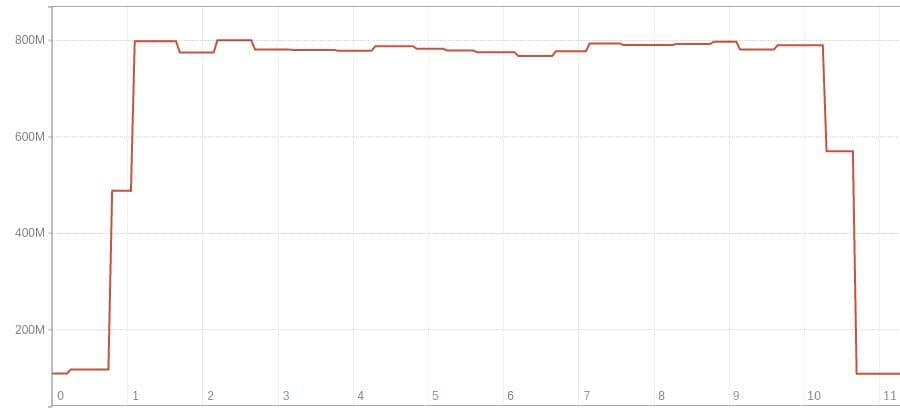
\includegraphics[width=\linewidth]{figures/experiment-figures/nursery_memory_usage.jpg}
    \captionof{figure}{nurseryschool}
    \end{subfigure}
    \hfill
    \begin{subfigure}{0.47\linewidth}
    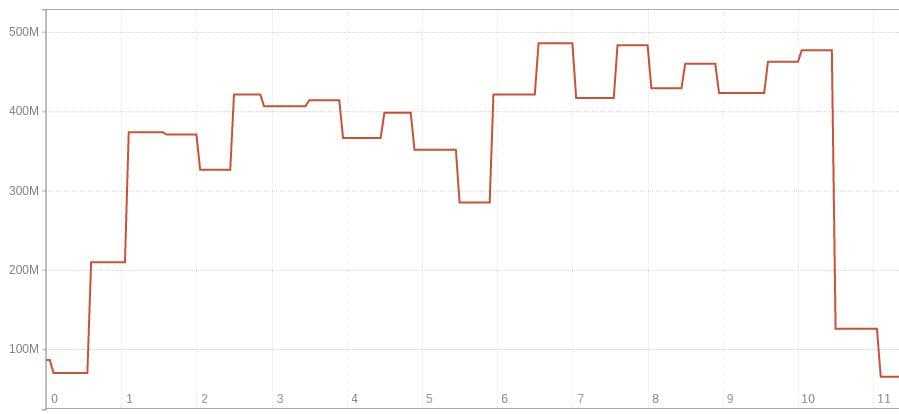
\includegraphics[width=\linewidth]{figures/experiment-figures/fluka_memory_usage.jpg}
    \captionof{figure}{fluka}
    \end{subfigure}
    \vspace{-1.5em}
    \caption{Memory use}
    \vspace{-1.5em}
    \label{fig:memory}
\end{figure}

\begin{wraptable}{r}{.5\textwidth}
    \centering
    \begin{tabular}{|l|ll|ll}
    \cline{1-3}
    \textbf{QoS} & \multicolumn{1}{l|}{\textbf{CPU}} & \textbf{RAM(MiB)} &  &  \\ \cline{1-3}
    test         & 0.3                                & 104               &  &  \\ \cline{1-1}
    standard     & 2.3                                & 257               &  &  \\ \cline{1-1}
    critical     & 3  & 800               &  &  \\ \cline{1-3}
    \end{tabular}
    \caption{\emph{Peak resource consumption per QoS during stress tests}}
    \label{table_of_resources}
    \vspace{-2em}
\end{wraptable}

\subsection{Optimized resource allocation vs. physical infrastructure}

Based on the results in section \ref{sec:measurements}, we can see that response time may vary between QoS but remain under acceptable values.
We can now estimate the baseline resources for the new infrastructure.
The Expected Load is the maximum load registered during the tests plus 25\% overhead.

The expected memory is:
\[
\begin{array}{rcl}
TotalMem & = & 1.25 * (C * L_c + S * L_s + T * L_t) \\
 & = & 20*1000MiB + 600*322MiB + 500*130MiB \\
 & = & 277750MiB  \approx  336GB
\end{array}
\]
Where:
\begin{conditions}
 L_i   & Expected max memory for each QoS class (table \ref{table_of_resources}) \\
 C     & Total number of Critical Websites \\
 S     & Total number of Standard Websites \\
 T     & Total number of Test Websites \\
\end{conditions}

The physical infrastructure has 2TB of memory. To meet our SLO, the memory estimate for the Kubernetes infrastructure is 336GB.
This is only \emph{16.8\% of the memory required in the physical infrastructure}, resulting in significant potential cost savings,
even disregarding cluster autoscaling.